\begin{frame}[t]{New kids: PhD Orientation Weekend Retreat}
  \begin{columns}
    \column{0.5\textwidth}
    \includegraphics[width=0.6\textheight]{media/powr}
    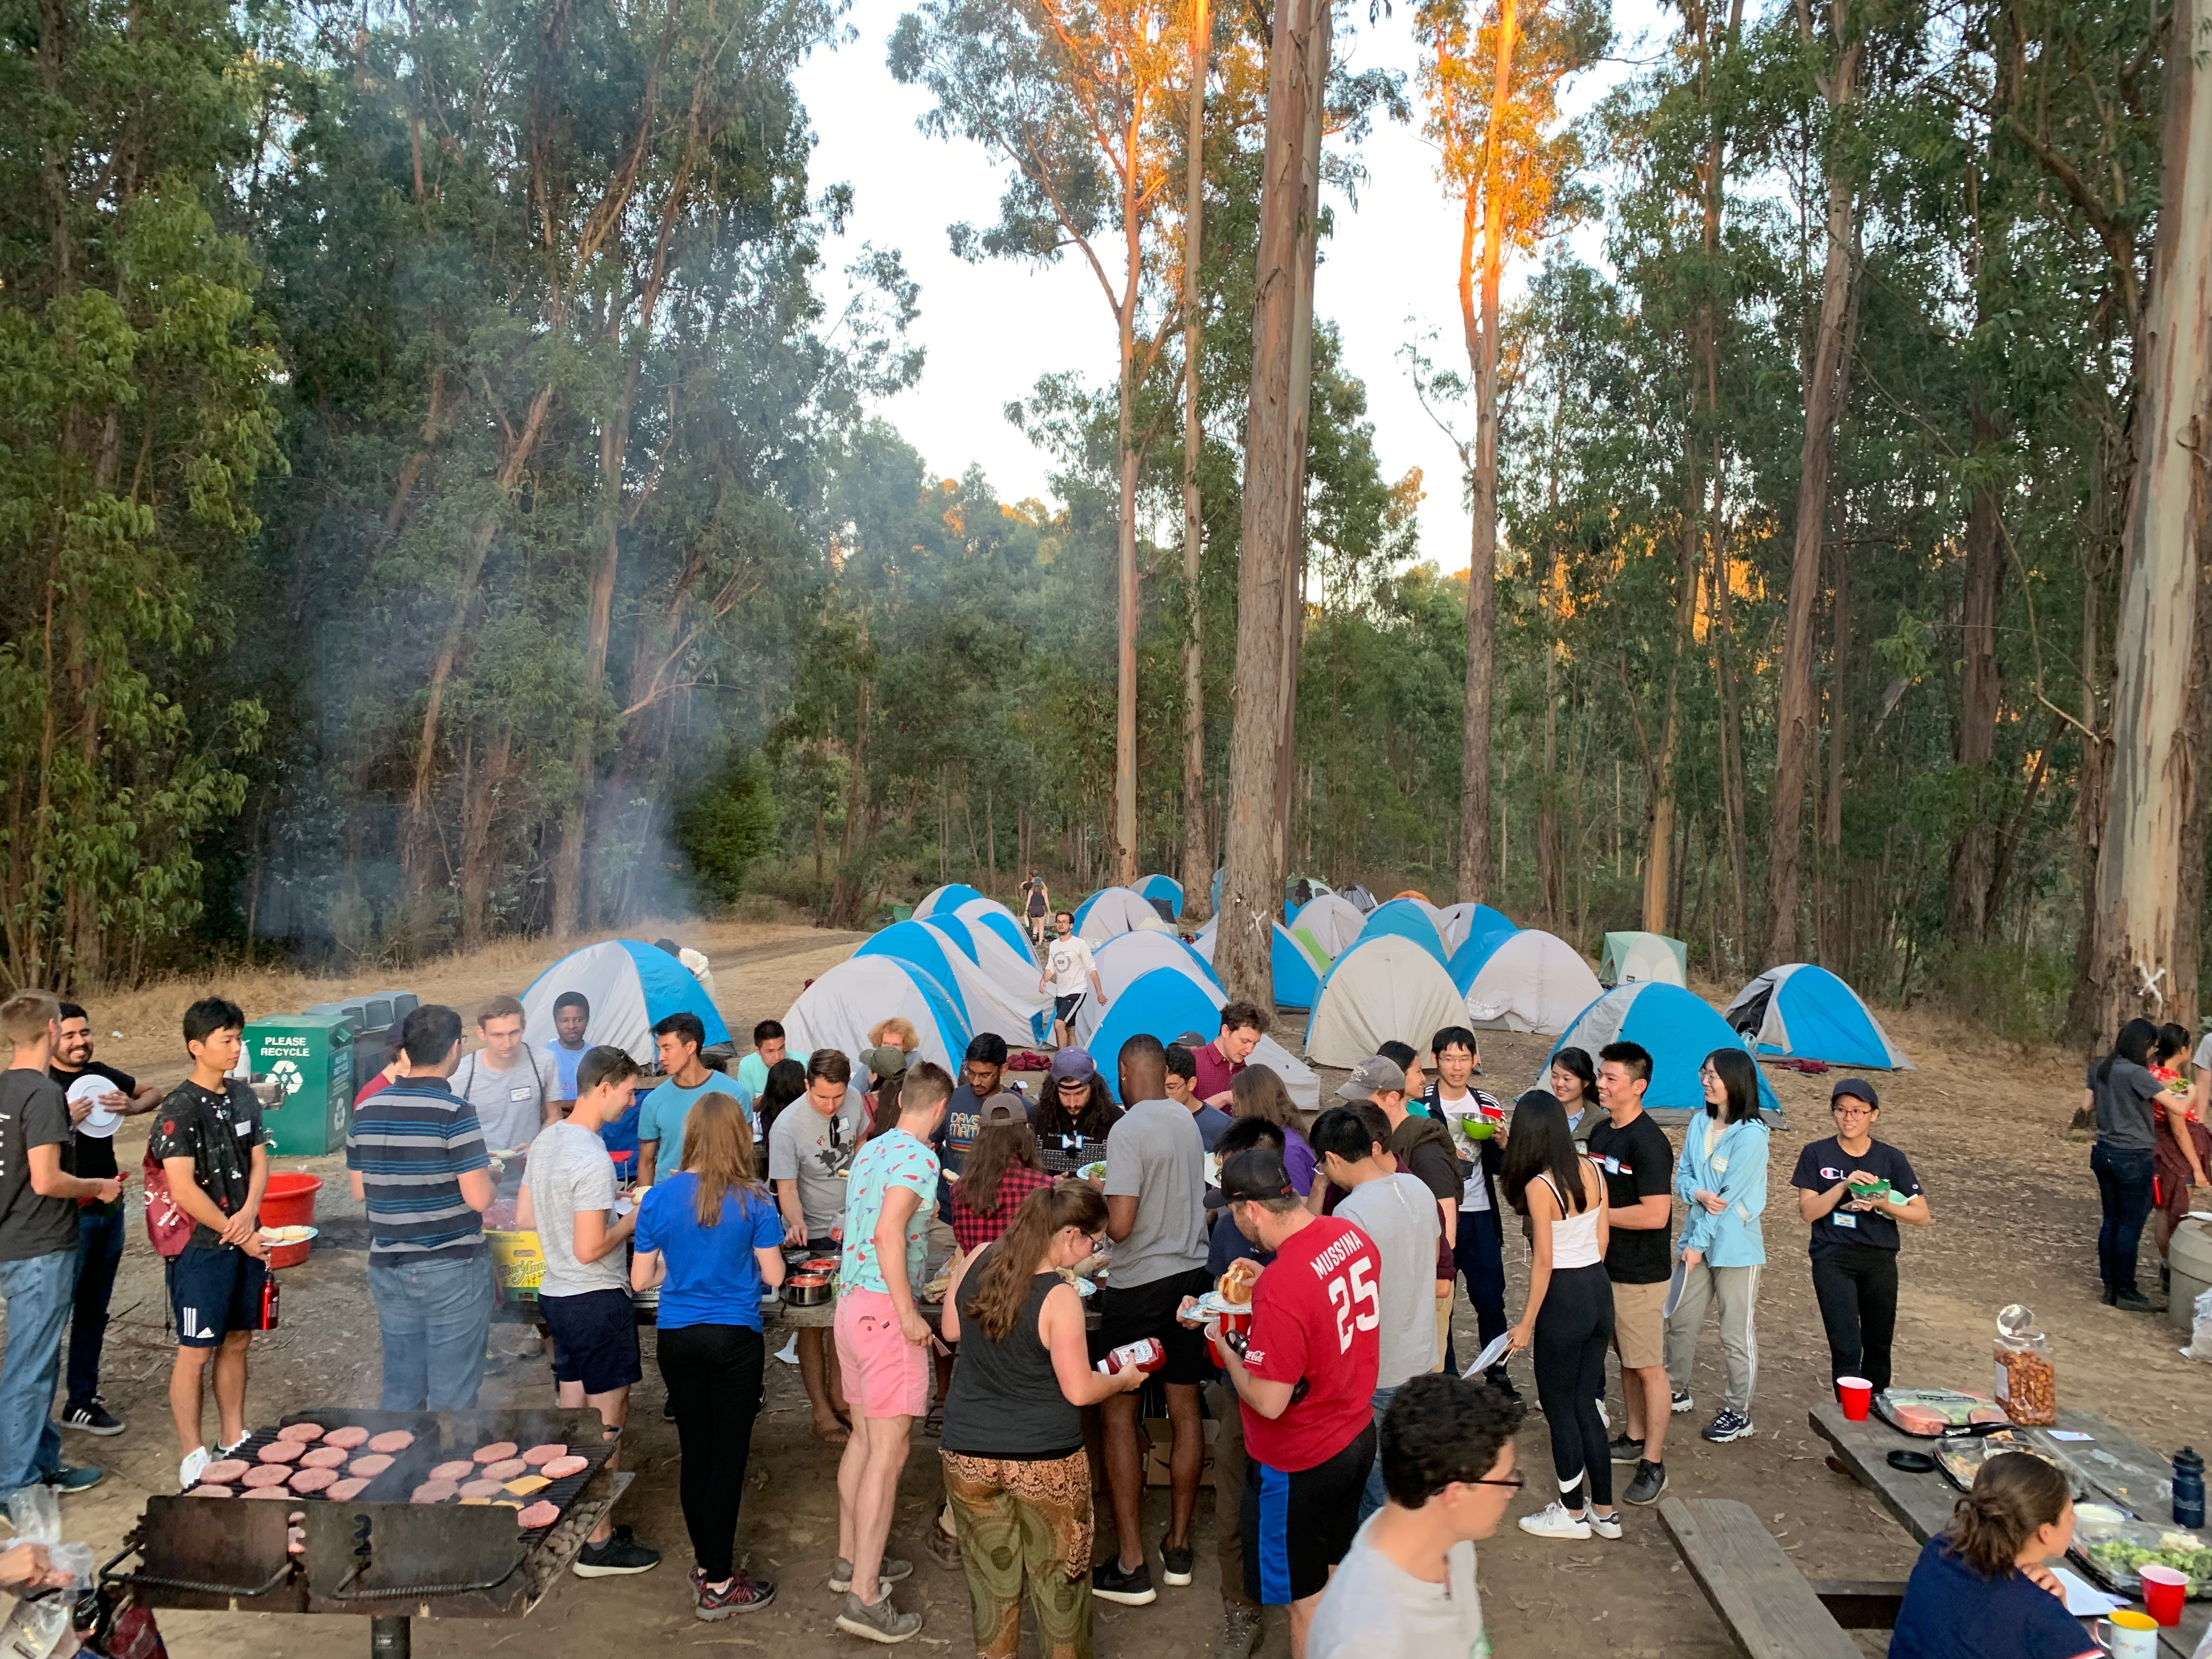
\includegraphics[width=0.6\textheight]{media/powr-meal}
    \column{0.5\textwidth}
    \includegraphics[width=0.5\textheight]{media/powr-gong}
  \end{columns}
\end{frame}
%--- Next Frame ---%

\begin{frame}{Whole-brain prediction facilitates construction of causal models}
  \begin{columns}[t]
    \column{0.31\textwidth}
    \uncover<1->{
      \resizebox{\textwidth}{!}{% \documentclass[tikz,crop]{standalone}
\documentclass[border=15pt, multi, tikz, ifthen, xcolor]{standalone}
\usepackage{tikz, xcolor, ifthen}
\usetikzlibrary{shapes,arrows}
\usetikzlibrary{positioning}

\begin{document}

\begin{tikzpicture}[node distance = 2cm, auto]
    \node [] (o1) {observations};
    \node [above=5mm of o1] (m1) {model};
    \node [above=5mm of m1] (b1) {biology};
    \path [line] (b1) -- (m1);
    \path [line] (m1) -- (o1);
\end{tikzpicture}
\end{document}
}
    }
    \column{0.65\textwidth}
    \only<2>{
      \resizebox{\textwidth}{!}{% \documentclass[tikz,crop]{standalone}
\documentclass[border=15pt, multi, tikz, ifthen, xcolor]{standalone}
\usepackage{tikz, xcolor, ifthen}
\usetikzlibrary{shapes,arrows}
\usetikzlibrary{positioning}

\begin{document}

\begin{tikzpicture}[node distance = 2cm, auto]
    \node [] (o1) {observations};
    \node [right=2mm of o1] (b1) {biology prior};
    \node [below right=5mm and -3mm of o1] (m1) {model};
    \node [below=5mm of m1] (b2) {biology posterior};
    \path [line] (o1) -- (m1);
    \path [line,dashed] (b1) -- (m1);
    \path [line,dashed] (m1) -- (b2);
\end{tikzpicture}
\end{document}
}
    }
    \only<3->{
      \resizebox{\textwidth}{!}{% \documentclass[tikz,crop]{standalone}
\documentclass[border=15pt, multi, tikz, ifthen, xcolor]{standalone}
\usepackage{tikz, xcolor, ifthen}
\usetikzlibrary{shapes,arrows}
\usetikzlibrary{positioning}

\begin{document}

\begin{tikzpicture}[node distance = 2cm, auto]
    \node [] (o1) {\emph{do}(observations)};
    \node [right=2mm of o1] (b1) {biology prior};
    \node [below right=5mm and -3mm of o1] (m1) {model};
    \node [below=5mm of m1] (b2) {biology posterior};
    \path [line] (o1) -- (m1);
    \path [line,dashed] (b1) -- (m1);
    \path [line,dashed] (m1) -- (b2);
\end{tikzpicture}
\end{document}
}
    }
  \end{columns}
  \uncover<4->{
    \begin{itemize}
      \item Observing whole-brain $\rightarrow$ fewer latent variables
      \item Interventions enable building causal model
      \item Causal models aid applications and interpretations
    \end{itemize}
  }
  \note[item]{Data-driven approach may result in empirically more accurate model.}
    \note<4->[item]{Behavior is encoded by populations of neurons distributed across whole-brain.}
\end{frame}

\begin{frame}{\aimOne}
  \textbf{\qOne}
  \begin{itemize}
    \item State-of-art performance in video prediction is achieved by deep generative models
    \item Initial modeling results suggest that spatial modeling out-performs traditional point process models of neurons on Calcium data
    \item Performed prototype analysis on voltage indicator data
  \end{itemize}
\end{frame}

\begin{frame}{\aimTwo}
  \textbf{\qTwo}
  \begin{itemize}
    \item For complex models fit to finite observations, multiple choices of parameters may perform equally well
    \item We can resolve this by testing if model substructures are causal with optogenetics
    \item ChRmine Tol2 injections show sparse expression, but behavioral signs of efficacy
  \end{itemize}
\end{frame}

\begin{frame}{\aimThree}
  \textbf{\qThree}
  \begin{itemize}
    \item \emph{in situ} hybridization (ISH) and connectome data contribute to understanding of colored graphs that underlie functional observations
    \item First attempt to add excitatory and inhibitory staining as an additional model input modestly hurt performance
    \item Experimented with training model to predict ISH data, with no success yet
    \item Known circuit motifs can be used as a prior, or we can try to discover structure using structure active learning
  \end{itemize}
\end{frame}
